% Metódy inžinierskej práce

\documentclass[10pt,oneside,slovak,a4paper]{article}

\usepackage[slovak]{babel}
%\usepackage[T1]{fontenc}
\usepackage[IL2]{fontenc} % lepšia sadzba písmena Ľ než v T1
\usepackage[utf8]{inputenc}
\usepackage{graphicx}
\usepackage{url} % príkaz \url na formátovanie URL
\usepackage{hyperref} % odkazy v texte budú aktívne (pri niektorých triedach dokumentov spôsobuje posun textu)

\usepackage{cite}
%\usepackage{times}

\pagestyle{headings}

\title{Rozvoj kritického myslenia s pomocou hier\thanks{Semestrálny projekt v predmete Metódy inžinierskej práce, ak. rok 2022/23, vedenie: Vladimír Mlynarovič}} % meno a priezvisko vyučujúceho na cvičeniach

\author{David Kolínek\\[2pt]
	{\small Slovenská technická univerzita v Bratislave}\\
	{\small Fakulta informatiky a informačných technológií}\\
	{\small \texttt{xkolinek@stuba.sk}}
	}

\date{\small 18 Október 2022 } % upravte



\begin{document}

\maketitle

\begin{abstract}
V tomto projekte by sme sa chceli zamerať na zmysel využitia hier v rannom veku aby zlepšili rozvoj 
detského mozgu v oblasti logického a kritického myslenia, ktoré je nesmierne dôležité ako pri štúdiu 
tak aj v každodennom živote. Mozog každého človeka kalkuluje pri každej situácii čo má vykonať aby 
z daných možností dosiahol požadovaného výsledku už od každodenných situácii ako je aj napríklad 
bežná komunikácia až po neskoršie náročné úlohy v akomkoľvek odvetví. Preto je našou úlohou zistiť 
čo najviac informácii o tom ako dokáže ľudský mozog benefitovať z precvičovania náročných situácii 
ktoré môžu aj hry môžu simulovať. Táto práca zpracuje využitie hier v bežných školách a výsledkoch po ich implementácii.
\end{abstract}



\section{Úvod}

Motivujte čitateľa a vysvetlite, o čom píšete. Úvod sa väčšinou nedelí na časti.

\section{Kritické myslenie}
Kritické myslenie je proces, pomocou ktorého ľudia dokážu sami hodnotiť rozličné
informácie. Ľudia, ktorí dokážu pri riešení rozličných problémov dospieť
k spoľahlivým záverom založených na faktoch, ktoré mali počas riešenia k dispozícii,
majú veľmi dobre vyvinutú schopnosť kriticky myslieť.
Ľudia s dobre vyvinutým kritickým myslením dokážu riešiť problémy bez pomoci
iných ľudí, pričom dospievajú k spoľahlivým záverom. V súčasnej dobe je veľmi
dôležité, aby učitelia počas vyučovacích hodín u žiakov rozvíjali schopnosť kriticky
myslieť a uvažovať Chápanie pojmu myslenie nie je jednotné. Väčšina odborníkov, ktorí sa zaoberajú
problematikou myslenia sa však zhodujú v tom, že myslenie predstavuje najvyššiu
formu poznávania a jeho podstatou je mentálna manipulácia so slovami
a predstavami zameraná na tvorbu pojmov, riešenie problémov a rozhodovanie.
Existuje viacero kritérií, podľa ktorých sa myslenie delí na jednotlivé druhy myslenia.
Podľa vývojového hľadiska sa myslenie delí na konkrétne a abstraktné; podľa smeru
myslenia vo vzťahu k abstraktnému a konkrétnemu na induktívne a deduktívne;
podľa počtu výsledkov myslenia pri riešení úloh na konvergentné a divergentné;
podľa stupňa systematickosti, dôslednosti, objektívnosti a kontroly procesu myslenia
na kritické a nekritické.

\section{Ako Hearts of iron 4 vie rozvíjať mysel a stratégiu}
\subsection{Čo je hearts of iron 4}
Hearts of Iron IV, známa aj ako HOI4, je grandiózna strategická počítačová vojnová hra, ktorú vyvinulo vývojárske štúdio Paradox a vydala spoločnosť Paradox Interactive. Celosvetovo bola vydaná 6. júna 2016 a je pokračovaním hry Hearts of Iron III z roku 2009 a štvrtým hlavným dielom série Hearts of Iron. Rovnako ako predchádzajúce hry v sérii, aj Hearts of Iron IV je grandiózna strategická vojnová hra, ktorá sa zameriava na druhú svetovú vojnu. Hráč môže prevziať kontrolu nad ľubovoľným národom na svete v roku 1936 alebo 1939 a viesť ho k víťazstvu alebo porážke proti iným krajinám.\\

Táto veľká strategická vojnová hra ponúka hlbokú historickú hrateľnosť aj lákavé alternatívne dejiny, keď sa na vašom počítači odohrávajú dramatické udalosti druhej svetovej vojny. Hearts of Iron IV je strhujúca simulácia modernej vojny, ktorá odmeňuje opakované hranie a strategické myslenie.\\

Hlavné funkcie:\\
Odmeňujúca strategická hrateľnosť:\\
Spravujte bojové fronty na celom kontinente a komplexný výskumný strom spolu s diplomaciou a politikou. Pripravte svoj národ na blížiacu sa búrku a transformujte geopolitickú krajinu vo svoj prospech.\\
Komplexná vojenská simulácia:\\
Vydávajte rozkazy armádnym skupinám zloženým z divízií podľa vlastného návrhu, ktoré smerujú k vašim cieľom a riadia zásobovacie línie. Pre celkový úspech je nevyhnutná koordinácia vzdušných, pozemných a námorných divízií.
Prevezmite kontrolu nad ktorýmkoľvek štátom:\\
Vyberte si jednu z najväčších mocností, ktoré sa snažia zvíťaziť, alebo sa postavte do úlohy jedného z menších národov, ktorý sa jednoducho snaží prežiť búrku.\\
Vnútorná politika:\\
Vyberte si vojnový kabinet podľa aktuálnych potrieb. Pred vojnou spravujte výskumníkov a priemyselníkov a po tom, čo sa svet neúprosne zosunie do konfliktu, klásť dôraz na vojenský kabinet.\\
Priemyselná moc: V rámci svojej stratégie sa zamerajte na priemyselnú moc:\\
Postavte továrne a prístavy a potom tieto štruktúry použite na výrobu všetkého, čo moderná armáda potrebuje. Plánujte múdro a vyvažujte budúce investície s aktuálnymi potrebami.\\
Posúvajte hranice vedy:\\
Flexibilný systém výskumu ponúka nové zbrane, nové priemyselné systémy a pokročilé strategické koncepty.\\
Intenzívny online boj:\\
Až 32 hráčov môže hrať Hearts of Iron IV, či už súťažne alebo kooperatívne, pričom niektorí hráči môžu prevziať kontrolu nad rôznymi aspektmi stratégie jedného národa.\\

\subsection{Stratégia k víťazstvu}
\section{Rast podnikateľského myslenia}

Použitie hry ako učebnej pomôcky sa od 90. rokov 20. storočia objavuje čím ďalej tým častejšie, pričom v dnešnej dobe enormného rozvoja pedagogických metód ale najmä v oblasti rozvoja podnikatelského myslenia.
Hry sa môžu používať v kombinácii s akoukoľvek inou pedagogikou na posilnenie jej 
efektívnosti definovanej ako: "Hravé hry sú pre žiakov veľmi dôležité:
...inovatívny prístup k učeniu odvodený od používania počítačových hier, ktoré majú 
vzdelávaciu hodnotu, alebo rôzne druhy softvérových aplikácií, ktoré využívajú hry na učenie a 
vzdelávacie účely, ako je podpora učenia, zlepšenie vyučovania, hodnotenie a posudzovanie žiakov (Tang, Hanneghan, Rhalibi, 2009, s. 3).
Výskum a štúdium podnikania ako disciplíny si v posledných desaťročiach udržali svoju 
v akademickom prostredí svoje vlastné miesto, dokonca predstihlo iné oblasti ekonomických štúdií vďaka neustálemu rastu 
záujmu o túto oblasť. Kolektívny význam podnikateľov, najmä v rámci rozvíjajúcich sa 
ekonomík štátov na celom svete (vrátane Slovenska), zdôrazňuje význam vzdelávania v oblasti podnikania pre ich občanov (Global Entrepreneurship Monitor [GEM], 2014). Podnikanie je kľúčom k hospodárskemu rastu krajiny (Faggian, Partridge a Malecki, 2016; Minniti, 
2008). Prognózy sa prikláňajú k tomu, že ekonomiky BRIC (Brazília, Rusko, India a Čína) do roku 2050 prekonajú veľké ekonomiky G7 (USA, Spojené kráľovstvo, Nemecko, Kanada, Francúzsko, Taliansko a Japonsko) 
a to vďaka podnikateľskému zmýšľaniu bežných ľudí v rozvojových krajinách BRIC (Jakovljevic, 2016; 
D. Wilson a Purushothaman, 2003). Možno by sa podnikateľské vzdelávanie nemalo považovať za 
za dôležité len pre študentov terciárneho vzdelávania, ale malo by zahŕňať aj študentov stredných škôl, aby 
poskytnúť príležitosť tým študentom, ktorí sa z nejakého dôvodu nemôžu zúčastniť na vysokoškolskom vzdelávaní.
\subsection{PODNIKATEĽSKÉ MYSLENIE V TRIEDE }
Uvedený počet univerzít a vysokých škôl v USA, ktoré ponúkali podnikateľské vzdelávanie ako súčasť 
v rámci svojich učebných osnov, sa zo skromných začiatkov, keď ich bolo v 70. rokoch minulého storočia len niekoľko desiatok, zvýšil na 
viac ako 1600 do konca 20. storočia (Katz, 2003) a odvtedy sa jeho počet zvýšil na 
2100 inštitúcií do roku 2010 (Seppanen a Gualtieri, 2012). Na úrovni K-12 bol v USA zaznamenaný pokrok, ktorý ukazuje, že v rokoch 2009 až 2015 sa počet škôl poskytujúcich štandardy, usmernenia alebo odborné znalosti zvýšil z 19 štátov na 42 štátov. V tom istom sedemročnom období sa počet 
stredných škôl, ktoré vyžadujú predmet podnikanie, zvýšil z 5 na 18 štátov (JAUSA, 2015).
V rozvojových krajinách počet škôl, ktoré ponúkajú podnikateľské programy, výrazne zaostáva 
Západu. Typickým príkladom je Vietnam. Podnikanie nie je súčasťou hlavných učebných osnov na národných univerzitách ani na stredných školách v celej krajine. Vykonávanie jednoduchého 
Internetové vyhľadávanie programov podnikania ponúkaných na terciárnej úrovni vo Vietname odhalí len 
len niekoľko výsledkov z inštitúcií najvyššej úrovne. Pokiaľ ide o tému podnikania, všeobecne 
nálada vysokoškolských študentov, ktorí sa zúčastnili prieskumu Global Entrepreneurship Monitor (GEM) 
v celom Vietname v roku 2014 bol ich "strach zo zlyhania" pri začatí podnikania z dôvodu nedostatočného podnikateľského alebo dokonca základného podnikateľského vzdelania. Počet študentov, ktorí uviedli tento pocit, je na úrovni 55  v porovnaní s ostatnými študentmi, ktorí sa zúčastnili prieskumu na celom svete, považovaný za veľmi vysoký pre túto demografickú skupinu v 
v spojení s ich pocitom, že majú len obmedzené podnikateľské schopnosti. "Jasne to ukazuje 
že Vietnam by mal vzdelávať a poskytovať ľuďom viac podnikateľských vedomostí, a to už od ich 
žiakmi a študentmi. A tým by pomohol mladým ľuďom, aby boli sebavedomejší pri zapájaní sa do podnikania." (GEM, 2014, s. 14).\cite{McDonald-ECTS}

B. Gullach a E. Gullach (2015) uvádzajú podstatné rozdiely medzi kritickým
a nekritickým myslením v tabuľke1 :
Tabuľka 1: Rozdiely medzi kritickým a nekritickým myslením.
\begin{table}[]
\begin{tabular}{|l|l|}
\hline
\textbf{Nekritické myslenie}                  & \textbf{Kritické myslenie}                               \\ \hline
Hádanie                                       & Odhadovanie                                              \\ \hline
Uprednostňovanie                              & Hodnotenie                                               \\ \hline
Viera                                         & Predpokladanie                                           \\ \hline
Zoskupovanie                                  & Kategorizovanie, klasifikácia                            \\ \hline
Asociovanie pojmov                            & Hľadanie princípov                                       \\ \hline
Domnienky                                     & Hypotézy                                                 \\ \hline
Názory bez ich zdôvodnovania                  & Zdôvodnené názory                                        \\ \hline
Usudzovanie bez kritérii                      & Usudzovanie na základe kritérií                          \\ \hline
Čierno-biele, povrchové videnie sveta         & Pestrofarebné videnie sveta, idúce do podstaty, do hĺbky \\ \hline
Iracionálne, nedôsledné                       & Racionálne, dôsledné                                     \\ \hline
Napodobňovanie, preberanie myšlienok od iných & Originálne myslenie                                      \\ \hline
Pasívne                                       & Aktívne                                                  \\ \hline
Unidisciplinárne                              & Interdisciplinárne                                       \\ \hline
Dogmatické                                    & Pátrajúce, skúmajúce                                     \\ \hline
Vágne vyjedarovanie                           & Precízne vyjadrovanie                                    \\ \hline
Egoistické, emocionálne                       & Nezaujaté, bez predsudkov a emócií                       \\ \hline
Snaha naučiť sa to, čo vymysleli iný          & Snaha naučiť sa myslieť                                  \\ \hline
\end{tabular}
\end{table}

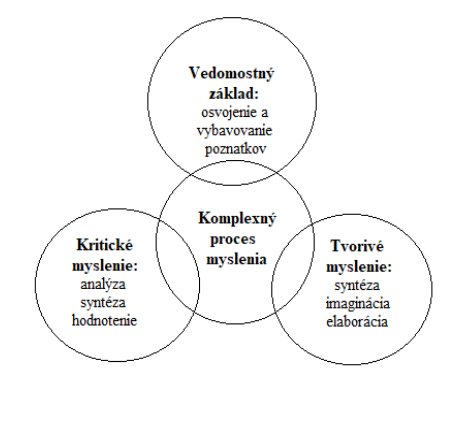
\includegraphics{RKM graf}

Obr. 1. Integrovaný model myslenia podľa Kollárikovej (zdroj: Kolláriková, 1995).\cite{KritickeATvoriveMyslenie}

\section{Iná časť} \label{ina}

Základným problémom je teda\ldots{} Najprv sa pozrieme na nejaké vysvetlenie (časť~\ref{ina:nejake}), a potom na ešte nejaké (časť~\ref{ina:nejake}).\footnote{Niekedy môžete potrebovať aj poznámku pod čiarou.}

Môže sa zdať, že problém vlastne nejestvuje\cite{Coplien:MPD}, ale bolo dokázané, že to tak nie je~\cite{Czarnecki:Staged, Czarnecki:Progress}. Napriek tomu, aj dnes na webe narazíme na všelijaké pochybné názory\cite{PLP-Framework}. Dôležité veci možno \emph{zdôrazniť kurzívou}. \cite{PLP-Framework}


\subsection{Nejaké vysvetlenie} \label{ina:nejake}

Niekedy treba uviesť zoznam:

\begin{itemize}
\item jedna vec
\item druhá vec
	\begin{itemize}
	\item x
	\item y
	\end{itemize}
\end{itemize}

Ten istý zoznam, len číslovaný:

\begin{enumerate}
\item jedna vec
\item druhá vec
	\begin{enumerate}
	\item x
	\item y
	\end{enumerate}
\end{enumerate}


\subsection{Ešte nejaké vysvetlenie} \label{ina:este}

\paragraph{Veľmi dôležitá poznámka.}
Niekedy je potrebné nadpisom označiť odsek. Text pokračuje hneď za nadpisom.
\cite{Djamas_Ramli}





% týmto sa generuje zoznam literatúry z obsahu súboru literatura.bib podľa toho, na čo sa v článku odkazujete
\bibliography{literatura}
\bibliographystyle{plain} % prípadne alpha, abbrv alebo hociktorý iný

\end{document}
